%%%%%%%%%%%%%%%%%%%%%%%%%%%%%%%%%%%%%%%%%%%%%%%%%%%%%%%%%%%%%%%%%%%%%%%%%%%%%%%%%%%%%%%%%%%%
\subsection*{Embedded System Design}
This section presents an overview of the embedded system design of the Aquapod, which has been split into three main components. Two of the printed circuit boards (PCBs) were custom designed to meet the volume restrictions while the third PCB was a small, COTS module. Splitting the electronics into separate boards allows the design to be highly versatile and expand with minimal effort. This also allowed for different sensor suites to be interchanged and made the robot more robust to ever adapting needs.

%%%%%%%%%%%%%%%%%%%%%%%%%%%%%%%%%%%%%%%%%%%%%%%%%%%%%%%%%%%%%%%%%%%%%%%%%%%%%%%%%%%%%%%%%%%%
\subsubsection*{Hardware Design}
The initial RC Aquapod had no embedded system design, and so the new iteration had to make a number of drastic changes. Due to the increase in internal components, space inside the robot was limited. A three-PCB design made up of a master board, a slave board, and a fuel-gauge board allowed the components to be broken apart and better utilize the space available. The complete system architecture can be seen in Figure \ref{fig:final-arch}.

%\begin{figure}[htc]
%finalized electrical architecture
\begin{figure}[ht]
	\begin{center}
		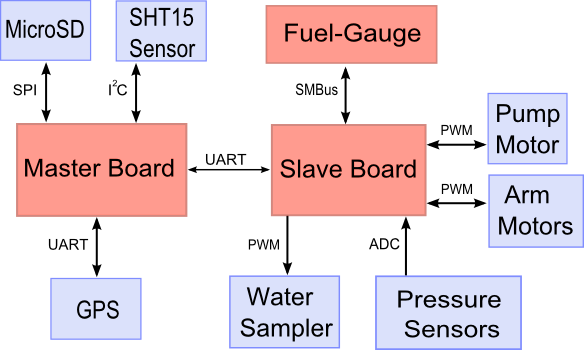
\includegraphics[width=1\columnwidth]{images/finalized-architecture2.png}
		\caption{Final embedded system architecture}
		\vspace{-20pt}
		\label{fig:final-arch}
	\end{center}
\end{figure}

%%%%%%%%%%%%%%%%%%%%%%%%%%%%%%%%%%%%%%%%%%%%%%
\subsubsection*{Master Board}
In order to facilitate the requirements within the time constraints, a COTS module was used for the master board. SparkFun Electronics sells this as the Package Tracker and runs on an LPC2148 ARM7 microcontroller. This unit was chosen for its 'ready to use' mircoSD card reader, onboard sensors, and GPS interface.  The master board is responsible for controlling the state machine of the robot, making decisions, and logging the sensor data.

\subsubsection*{Slave Board}
Due to the custom nature of the hardware, the slave board was designed specifically for the Aquapod robot. The main processor was chosen as the PIC16F1827 from MicroChip based on the number of required input and output pins. The slave board also includes a pressure sensor, charge recognition circuitry, communication devices, and the required motor drivers for five separate actuators (two arms, two samplers, and one pump). This board facilitates the low-level control of the motors and sensors, however, it will only act on commands sent by the master board.

%%%%%%%%%%%%%%%%%%%%%%%%%%%%%%%%%%%%%%%%%%%%%%
\subsubsection*{Sensors}
The Aquapod has two absolute pressure sensors with an output range of 0.3V to 4.9V, corresponding to an input range of 3 psi\(_a\) to 42 psi\(_a\), respectively. These sensors are used to monitor internal and external pressure and act as the main decision points of the state machine.

The two arm motors feature absolute magnetic shaft encoders to report the current arm position back the slave board which handles the PID control for arm movement. The pump motor also includes a digital encoder to determine the total water volume pumped into the bladder. The sampler motors have no feedback, but operate on a standard servo open-loop signal.

The COTS master board contains a number of onboard sensors including temperature, humidity, and a 3-axis accelerometer. The board can also access the SiRF III GPS module from USGlobalSat.

By communicating with the slave board, the master board is capable of measuring and logging all of these sensor values in a central log file and can make decisions based on the returned values, this will be discussed in more detail below.
%%%%%%%%%%%%%%%%%%%%%%%%%%%%%%%%%%%%%%%%%%%%%%
\subsection*{Power Architecture}
The Aquapods's power system comprises of three main parts: the battery and fuel-gauge, the battery charger, and the various power conversion electronics.  Wiring to chassis-mounted electronic components and high DC current lines is realized using twisted-pairs to increase noise immunity by reducing destructive (or unbalanced) effects resulting from electromagnetic interference coupled signals and ground return paths.

%\subsubsection*{Battery and Fuel-Gauge}
%\label{sec:batt_mgmt_and_gg}
At the heart of the robot's power system is a dedicated fuel-gauging chipset, described in \cite{Kottas2009}.  It provides all the necessary features to safely monitor any lithium-ion battery chemistry's dynamics, while tracking cell (capacity) degradation over time.  The resultant smart-battery system (SBS) is compliant with SBS v1.1 standards \cite{sbs_std}, and can report a wide array of static and dynamic battery parameters while idle, charging, or discharging to a host processor - in this case, the slave and master boards. This system is shown in Figure \ref{fig:pwr_blk_diag}.

A lithium-ion polymer battery (LiPB) was chosen to power the robot.  This particular battery chemistry was selected due to its thin and light-weight packaging, high energy density and output power capabilities.  It can source roughly 14Wh of energy, and satisfies the robot's operating time requirements. 

A highly integrated LiPB switch-mode charge-management circuit is included on slave board.  It is configured to charge the LiPB pack quickly and safely and contains a pre-charge (conditioning) mode for deeply discharged batteries.

\begin{figure}%
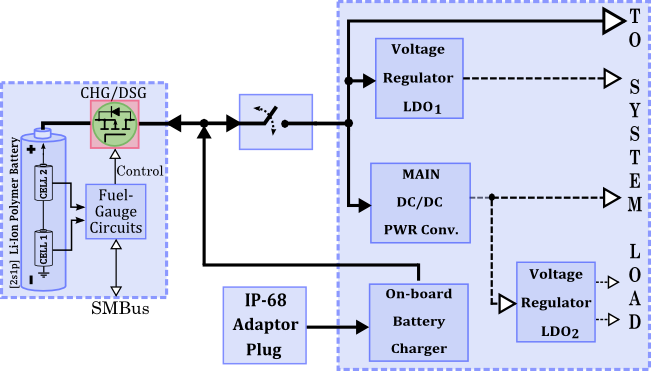
\includegraphics[width=1\columnwidth]{images/Aqua-Pod_Robot_PwrSys_Fig01.png}%
\caption{High-level power system block diagram}%
\vspace{-10pt}
\label{fig:pwr_blk_diag}%
\end{figure}

%%%%%%%%%%%%%%%%%%%%%%%%%%%%%%%%%%%%%%%%%%%%%%
\subsubsection*{Communication Protocol}
Command and Acknowledgment (CMD/ACK) messages are used to exchange data and commands between the boards. This hand-shaking protocol was enforced to ensure important commands from the master board were being process and executed by the slave board before continuing with the state machine. The master board can send one command at a time in a 9-byte packet to the slave board which will execute the command or return sensor values appropriately.  
%%%%%%%%%%%%%%%%%%%%%%%%%%%%%%%%%%%%%%%%%%%%%%
\subsection*{State Machine and Operational Profiles}
The main purpose for this version of the Aquapod was to collect water samples at a pre-programmed depth. Using a graphical user interface, the Aquapod can be programmed into one of four modes, including: Instant Dive(1), Remote Dive(2), Land Mode(3), and Purge Bladder(4). Selecting one of these modes will route the robot through the state machine which can be seen in Figure \ref{fig:Statemachine}.

\begin{figure}
	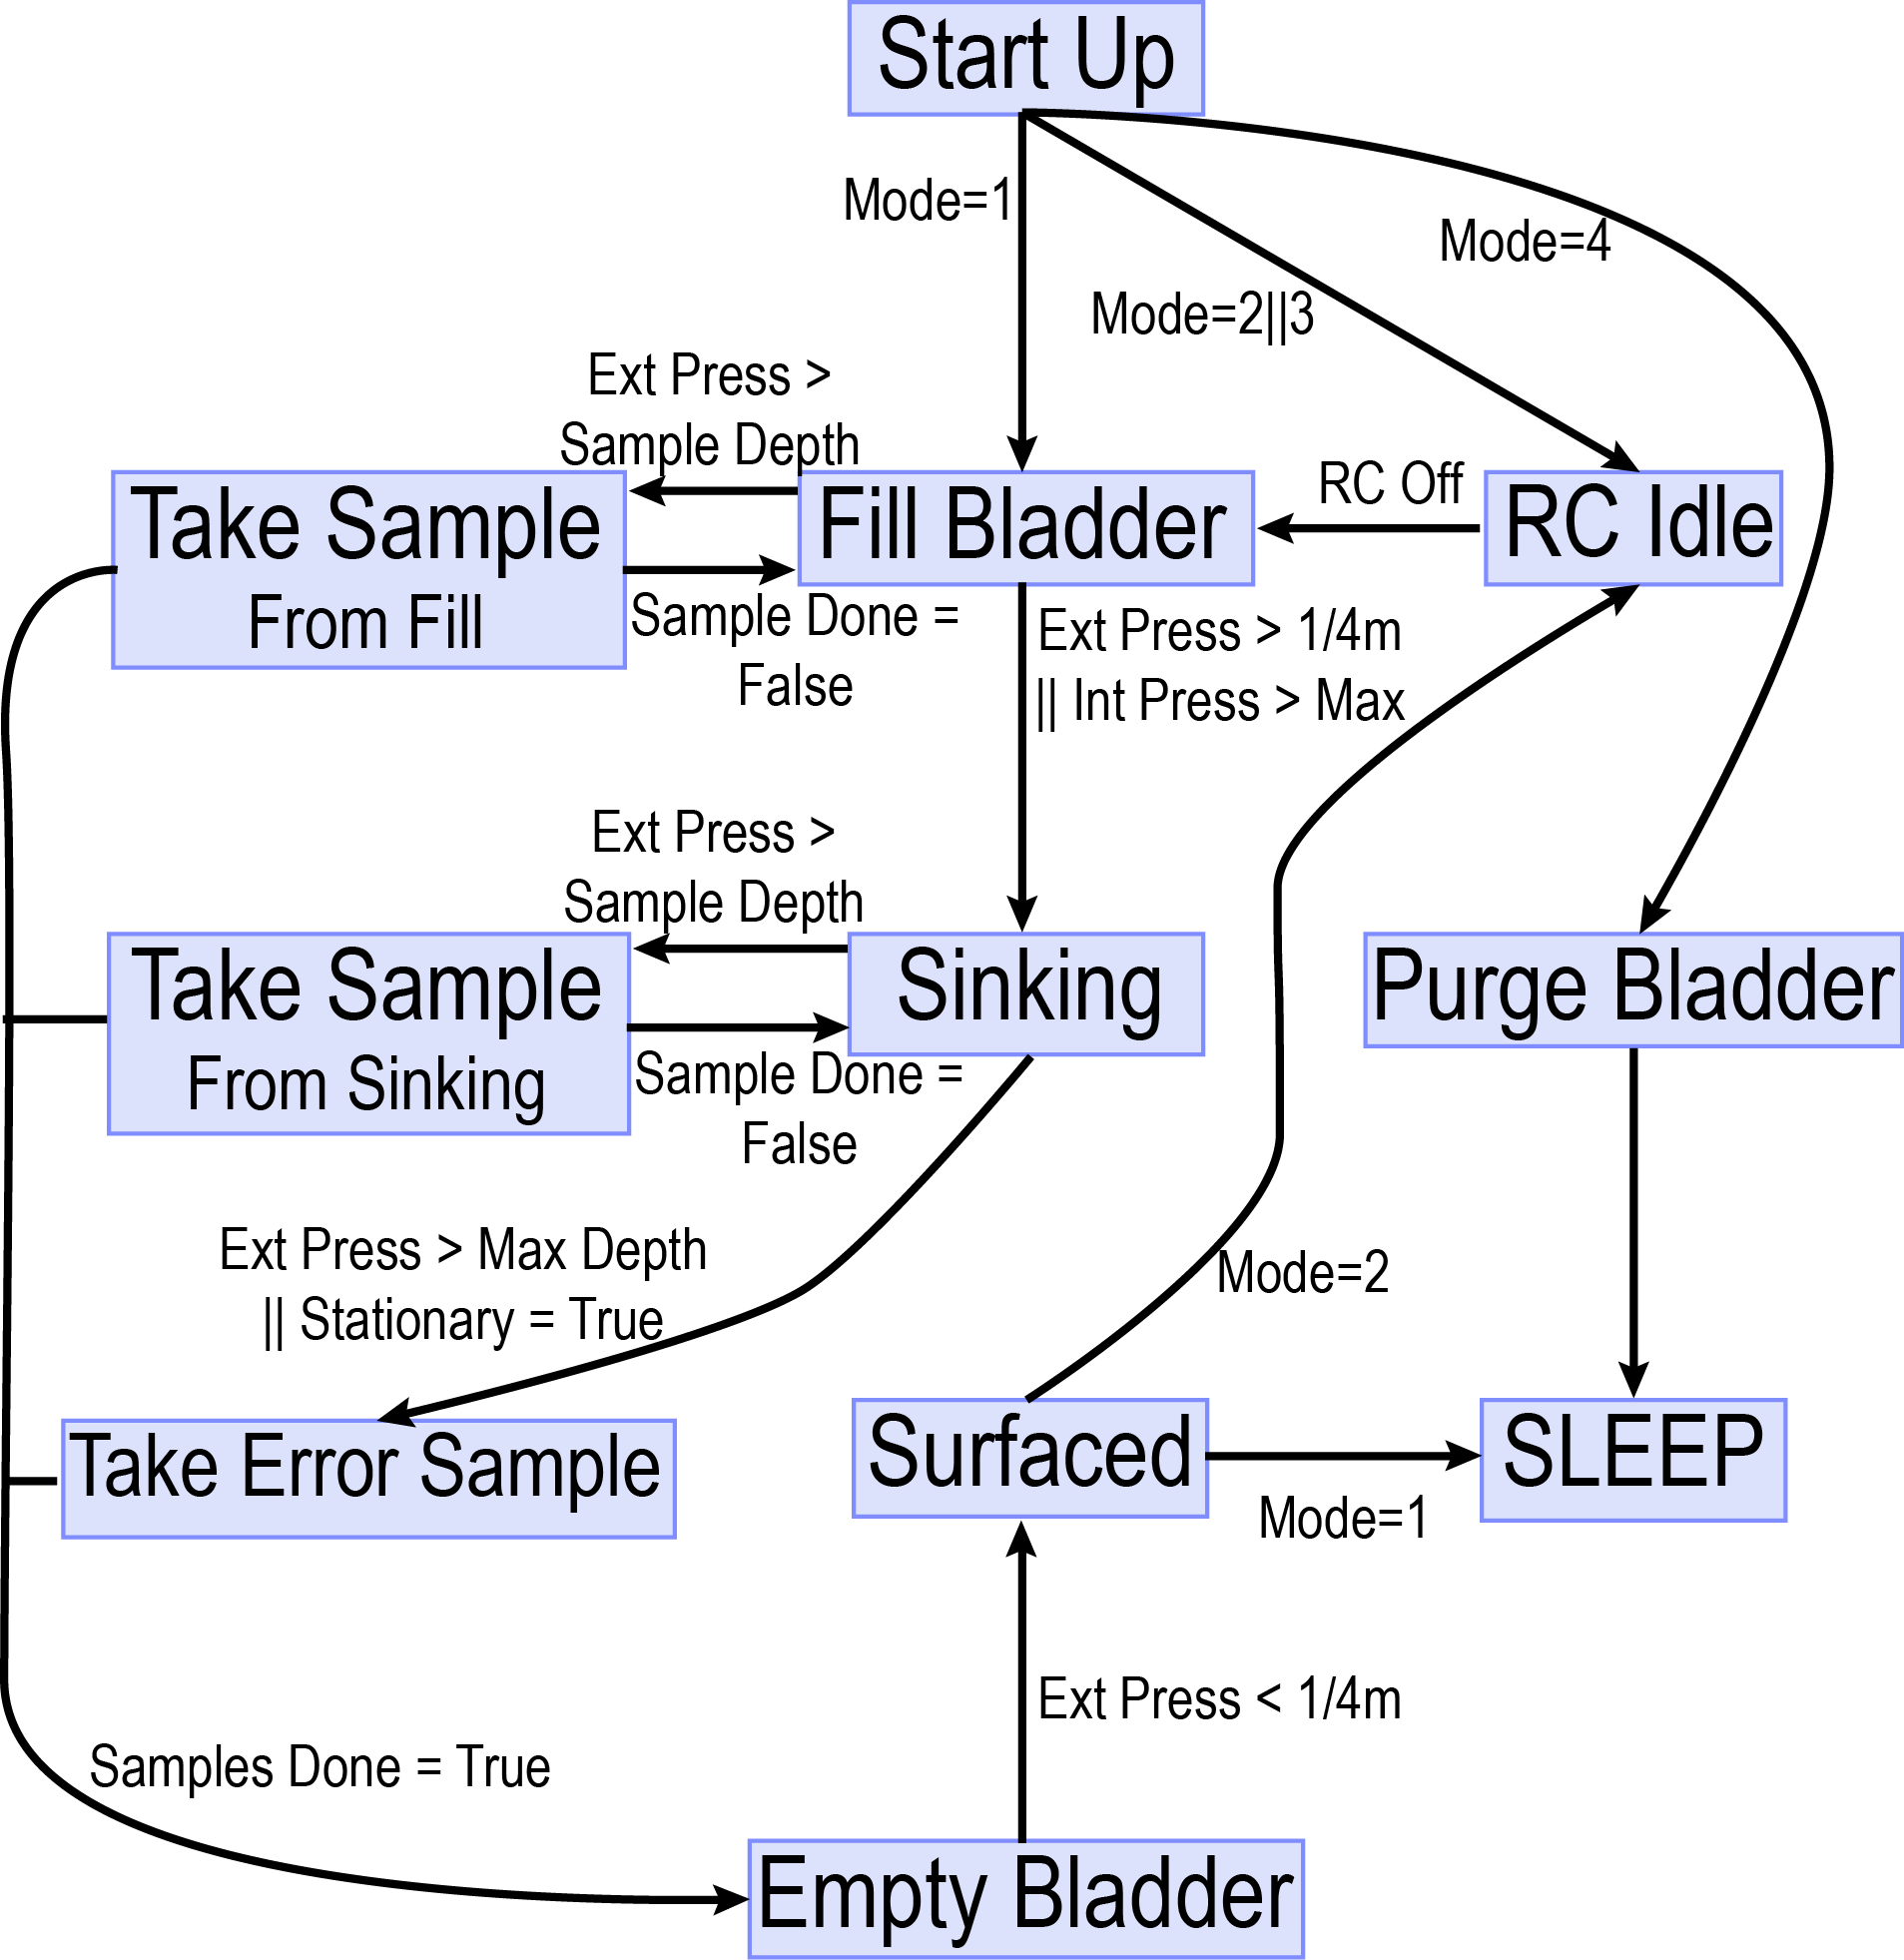
\includegraphics[width=1\columnwidth]{images/Statemachine.png}
	\caption{Aquapod state machine diagram}
	\vspace{-10pt}
	\label{fig:Statemachine}
\end{figure}

It was important to program a number of safety checks within the state machine to ensure that the robot will always resurface. Errors in the operation could include reaching a depth greater than 10m or hitting a surface before reaching the target depth. If one of these errors occurs, the robot will take a sample and return to the surface. Other system error checks were written directly into the slave board in case one of the boards reset, a sensor failure occurs, or other unlikely mishaps happen.

During either mode 2 or 3, the remote control (RC) operation is run. This allows the user to control the arms of the robot through a standard radio transmitter. In these modes the user can command the robot to tumbling to a particular location and dive or simply move around on land.

The state machine featured in Figure \ref{fig:Statemachine} is by no means extensive of the robot's capabilities. Further development and inclusion of the GPS module can greatly increase the functionality of the robot. This operation profile was simply used as an example for diving/sampling and as a demonstration tool. Autonomous control for long-term and unmonitored missions is feasible with the current hardware.

